\textbf{COLUNI 2023 -- Questão 22}\par\medskip Leia o texto a seguir.

\begin{center}\textbf{Beyond Visible Light}\end{center}
The rainbow of light that the human eye can see is a small portion of the total range of light, known in science as the electromagnetic spectrum. Telescopes can be engineered to detect light outside the visible range to show us otherwise hidden regions of space. The James Webb Space Telescope detects near-infrared and mid-infrared wavelengths, the light beyond the red end of the visible spectrum. Infrared light reveals new details in images, deepening our understanding of celestial objects.

% COLUNI-AUTO-FIGURES-BEGIN
\begin{figure}[htbp]
\centering
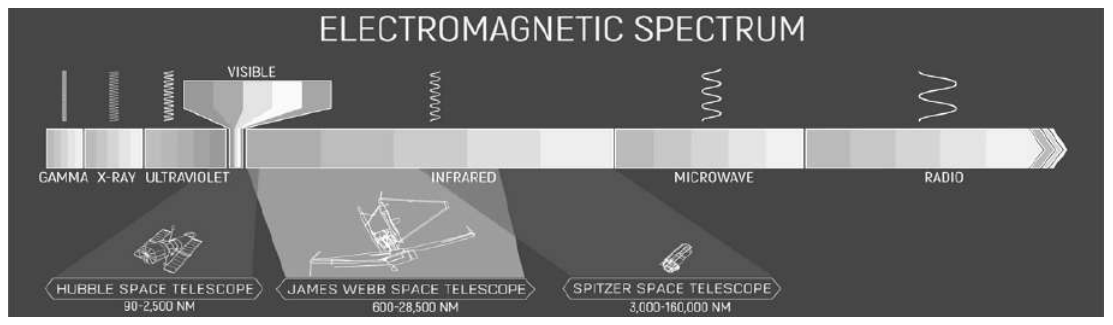
\includegraphics[width=0.95\linewidth]{static/simulados/coluni/figuras/2023/questao-21/figura-1.png}
\end{figure}
% COLUNI-AUTO-FIGURES-END
\begin{center}CREDIT: NASA and J. Olmsted [STScI].\end{center}

\textbf{About This Image}

This infographic illustrates the spectrum of electromagnetic energy, specifically highlighting the portions detected by NASA’s Hubble, Spitzer, and Webb space telescopes. The portion of the spectrum labeled “visible,” with the colors of the rainbow, is what humans detect as visible light. Beyond the red end of the visible spectrum, the wavelengths are longer than the human eye can detect. The portion of the spectrum immediately beyond red is called infrared. Humans can feel infrared energy as heat. Each of these telescopes detects portions of the infrared spectrum and astronomers can analyze that data, essentially making the invisible visible. Longer wavelengths like infrared, microwave, and radio waves are able to pass through areas of dense gas clouds and other matter in the universe where shorter wavelengths get trapped. By detecting these longer wavelengths with telescopes, we are able to see things in the universe that we could never see in visible light. The infographic demonstrates how much of the electromagnetic spectrum each of these telescopes covers and also their combined coverage. There are other telescopes that detect other portions of the electromagnetic spectrum, and together these scientific instruments give us a more complete picture of the universe and how it functions.

Disponível em: <https://webbtelescope.org/webb-science/the-observatory/infrared-astronomy>. Acesso em: 25 Ago. 2022.

\par\medskip Analise as afirmativas a seguir:

I. The verb \textbf{can} in the sentence: “[…] astronomers can analyze that data essentially making the invisible visible” expresses possibility.

II. The word \textbf{longer} in the sentence: “[…] the wavelengths are longer than the human eye can detect” is an example of an adjective in the superlative form.

III. The word \textbf{it} in the sentence: “[…] these scientific instruments give us a more complete picture of the universe and how it functions” substitutes the word universe.

Está CORRETO o que se afirma em:
\begin{enumerate}
\item I, II e III.
\item I e II, apenas.
\item II e III, apenas.
\item I e III, apenas.
\end{enumerate}
